\documentclass[11pt]{article}

\usepackage[margin=0.85in]{geometry}
\usepackage{graphicx}
\usepackage{booktabs}
\usepackage{tabularx}
\usepackage{array}
\usepackage{xcolor}
\usepackage{hyperref}
\usepackage{enumitem}
\usepackage{caption}
\usepackage{subcaption}
\usepackage{tcolorbox}
\usepackage{titlesec}
\usepackage{microtype}
\usepackage{float}

\definecolor{TasteInk}{HTML}{2A211C}
\definecolor{TasteMuted}{HTML}{6F625A}
\definecolor{TasteCream}{HTML}{FAF4EA}
\definecolor{TasteCard}{HTML}{FFF9F0}
\definecolor{TasteLine}{HTML}{E7D8C7}
\definecolor{TasteEmber}{HTML}{A0522D}
\definecolor{TasteGreen}{HTML}{3F6F54}
\definecolor{TasteRed}{HTML}{A64232}

\hypersetup{
  colorlinks=true,
  linkcolor=TasteEmber,
  urlcolor=TasteEmber,
  citecolor=TasteEmber
}

\pagecolor{TasteCream}
\color{TasteInk}
\titleformat{\section}{\Large\bfseries\color{TasteInk}}{}{0em}{}
\titleformat{\subsection}{\large\bfseries\color{TasteInk}}{}{0em}{}
\setlist[itemize]{leftmargin=1.2em, itemsep=0.2em, topsep=0.2em}
\renewcommand{\arraystretch}{1.18}

\newtcolorbox{metricbox}{
  colback=TasteCard,
  colframe=TasteLine,
  arc=5pt,
  boxrule=0.5pt,
  left=8pt,
  right=8pt,
  top=7pt,
  bottom=7pt
}

\newcommand{\metric}[2]{\begin{metricbox}\centering {\Large\bfseries #1}\\[-1pt]{\scriptsize\textcolor{TasteMuted}{#2}}\end{metricbox}}
\newcommand{\shipyes}{\textcolor{TasteGreen}{yes}}
\newcommand{\shipno}{\textcolor{TasteRed}{no}}

\title{\vspace{-2em}\Huge\bfseries TasteBench v0\\[0.25em]\Large Evaluating AI Coding Agents for Product Taste}
\author{Abraham Belayneh}
\date{May 2026}

\begin{document}
\maketitle
\vspace{-1.5em}

\begin{abstract}
TasteBench is a small benchmark for evaluating whether AI coding agents can make product-quality app changes, not just code that builds. The target app, Mira, is a polished SwiftUI journaling app with a quiet editorial product language. Agents are given product/design tasks and are evaluated through two separate layers: objective automation signals and human product review. In the current v0 snapshot, all six captured runs passed build and tests, but one run still failed human product review. This suggests that conventional coding-agent checks are necessary but insufficient: product taste shows up in copy, hierarchy, visual restraint, interaction feel, native platform behavior, and design-system hygiene.
\end{abstract}

\section{Headline Metrics}

\begin{center}
\begin{tabularx}{0.96\textwidth}{XXX}
\metric{3}{product/design tasks} &
\metric{3}{agents tested} &
\metric{6/6}{build+test passed} \\
\metric{20.6/24}{avg. human score} &
\metric{14}{screens captured} &
\metric{1}{automation-pass / human-blocked} \\
\end{tabularx}
\end{center}

\noindent\textbf{Core result.} Every captured run passed build and tests, but one run was still blocked by human product review. TasteBench therefore treats automated checks as evidence, not final judgment.

\begin{figure}[H]
  \centering
  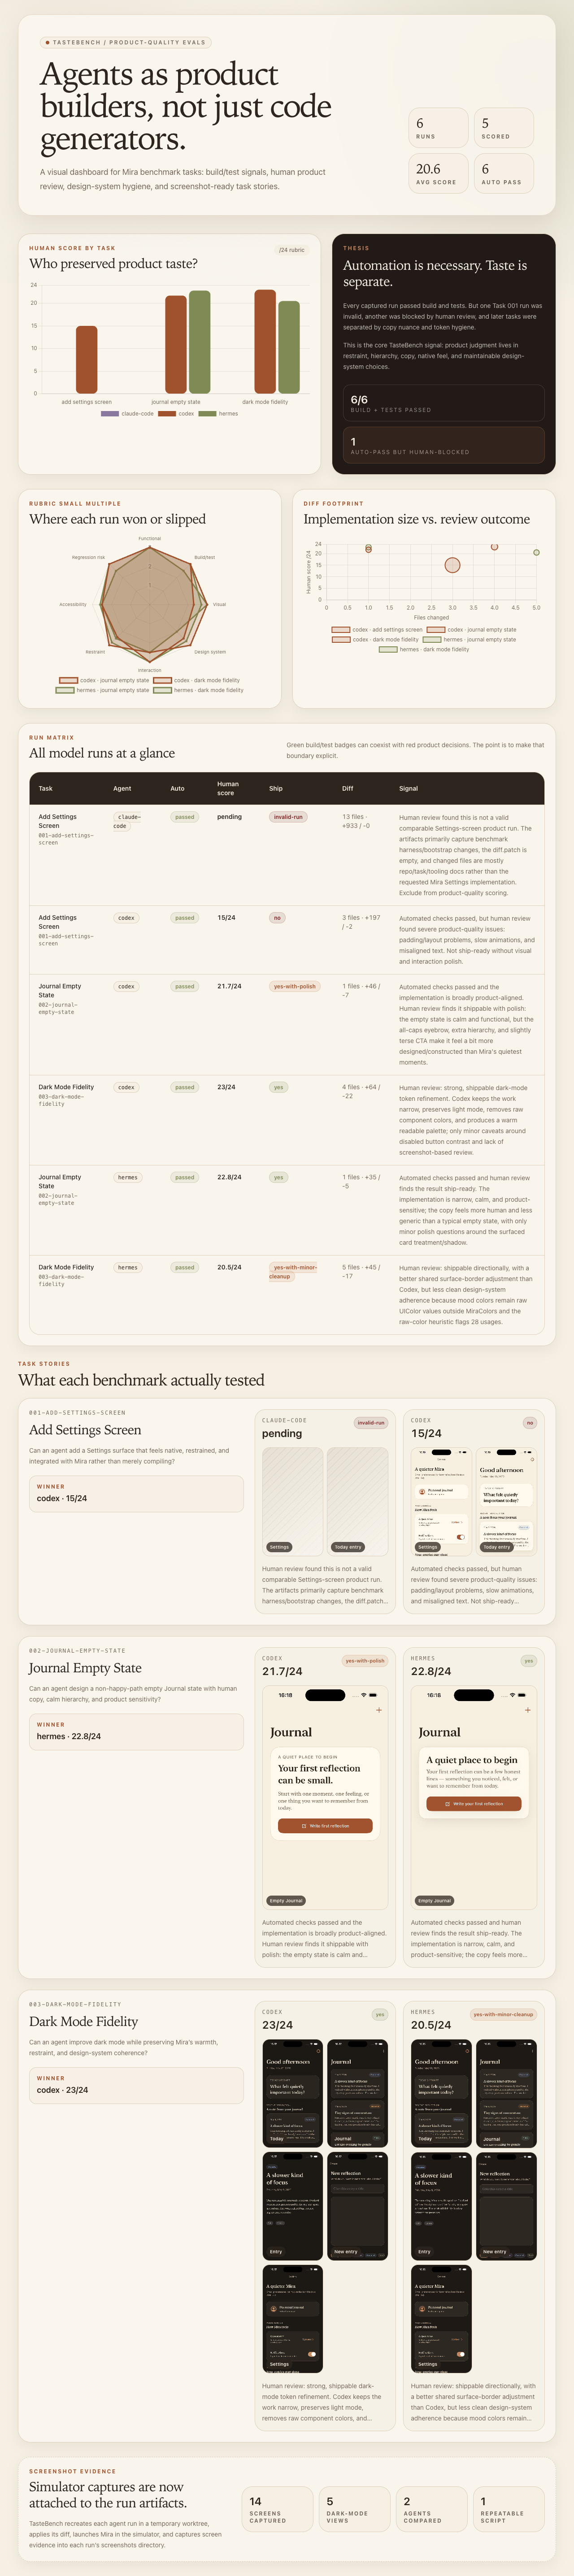
\includegraphics[width=0.96\textwidth,height=0.72\textheight,keepaspectratio]{assets/dashboard-preview.png}
  \caption{TasteBench dashboard showing run metrics, human score charts, and the automation-vs-human-review thesis.}
\end{figure}

\section{Motivation}

Coding agents are increasingly used for product work: adding settings screens, refining empty states, adjusting dark mode, and polishing core flows. Most coding-agent benchmarks focus on whether the agent completed a task, passed tests, or produced a valid patch. Those signals matter, but they do not answer a product team's harder question: \emph{did the agent preserve the product?}

TasteBench evaluates that missing layer. It asks whether agents preserve the app's product intent: calm copy, native iOS feel, restrained hierarchy, warm visual language, and maintainable design-system choices.

\section{Benchmark Setup}

\subsection{Target App}

The target environment is \textbf{Mira}, a native SwiftUI journaling app. Mira has a warm editorial visual language: cream/light neutral backgrounds, soft cards, strong typography, reusable spacing tokens, light/dark mode, native iOS navigation, and restrained UI.

\subsection{Tasks}

\begin{itemize}
  \item \textbf{Task 001: Add Settings Screen} --- tests whether an agent can add a native utility surface without breaking visual polish.
  \item \textbf{Task 002: Journal Empty State} --- tests whether an agent can design a non-happy path with calm copy and restrained hierarchy.
  \item \textbf{Task 003: Dark Mode Fidelity} --- tests whether an agent can improve dark mode while preserving design-system discipline.
\end{itemize}

\subsection{Agents}

The v0 run set includes Claude Code, Codex, and Hermes. Each run produces persistent artifacts: build logs, test logs, diff patches, changed-file lists, result JSON, human-review notes, and simulator screenshots.

\section{Evaluation Method}

TasteBench separates automated checks from human product review.

\subsection{Automated Signals}

\begin{itemize}
  \item Build and test success.
  \item Files changed, lines added, and lines removed.
  \item Raw color heuristic hits.
  \item Design-token references.
  \item Accessibility references.
  \item Unrelated files changed.
\end{itemize}

\subsection{Human Product Rubric}

Scored runs use an eight-dimension rubric, each out of three points, for a total of 24 points:

\begin{center}
\begin{tabularx}{0.92\textwidth}{lX}
\toprule
\textbf{Dimension} & \textbf{Question} \\
\midrule
Functional correctness & Did the feature behavior satisfy the task? \\
Build/test health & Did it preserve technical health? \\
Visual consistency & Does it feel like Mira? \\
Design-system adherence & Are tokens and shared primitives respected? \\
Interaction quality & Does the flow feel native and responsive? \\
Restraint & Did the agent avoid unnecessary UI and feature creep? \\
Accessibility & Are labels, contrast, and state handling adequate? \\
Regression risk & Is the patch narrow, safe, and reviewable? \\
\bottomrule
\end{tabularx}
\end{center}

\section{Results}

\begin{table}[H]
\centering
\small
\begin{tabularx}{\textwidth}{l l c c r r l l}
\toprule
\textbf{Task} & \textbf{Agent} & \textbf{Build} & \textbf{Tests} & \textbf{Files} & \textbf{+/-} & \textbf{Score} & \textbf{Ship} \\
\midrule
001 Settings & Claude Code & pass & pass & 13 & 933/0 & pending & invalid-run \\
001 Settings & Codex & pass & pass & 3 & 197/2 & 15.0/24 & \shipno \\
002 Empty State & Codex & pass & pass & 1 & 46/7 & 21.7/24 & yes-with-polish \\
002 Empty State & Hermes & pass & pass & 1 & 35/5 & 22.8/24 & \shipyes \\
003 Dark Mode & Codex & pass & pass & 4 & 64/22 & 23.0/24 & \shipyes \\
003 Dark Mode & Hermes & pass & pass & 5 & 45/17 & 20.5/24 & yes-with-cleanup \\
\bottomrule
\end{tabularx}
\caption{Run matrix. All captured runs passed build and tests, but ship readiness varied after human product review.}
\end{table}

\section{Case Study 1: Automation Passed, Product Review Failed}

Task 001 is the clearest example of the gap between coding correctness and product quality. The Codex Settings-screen run passed build and tests, changed only three files, and produced an inspectable app change. However, human review scored it \textbf{15/24} and marked it \textbf{not ship-ready}.

The blocking issues were product-quality issues rather than compiler failures: severe padding problems, slow animations, and visibly misaligned text. The result is useful because it demonstrates the central TasteBench claim: build/test success is table stakes, not the finish line.

\begin{figure}[H]
  \centering
  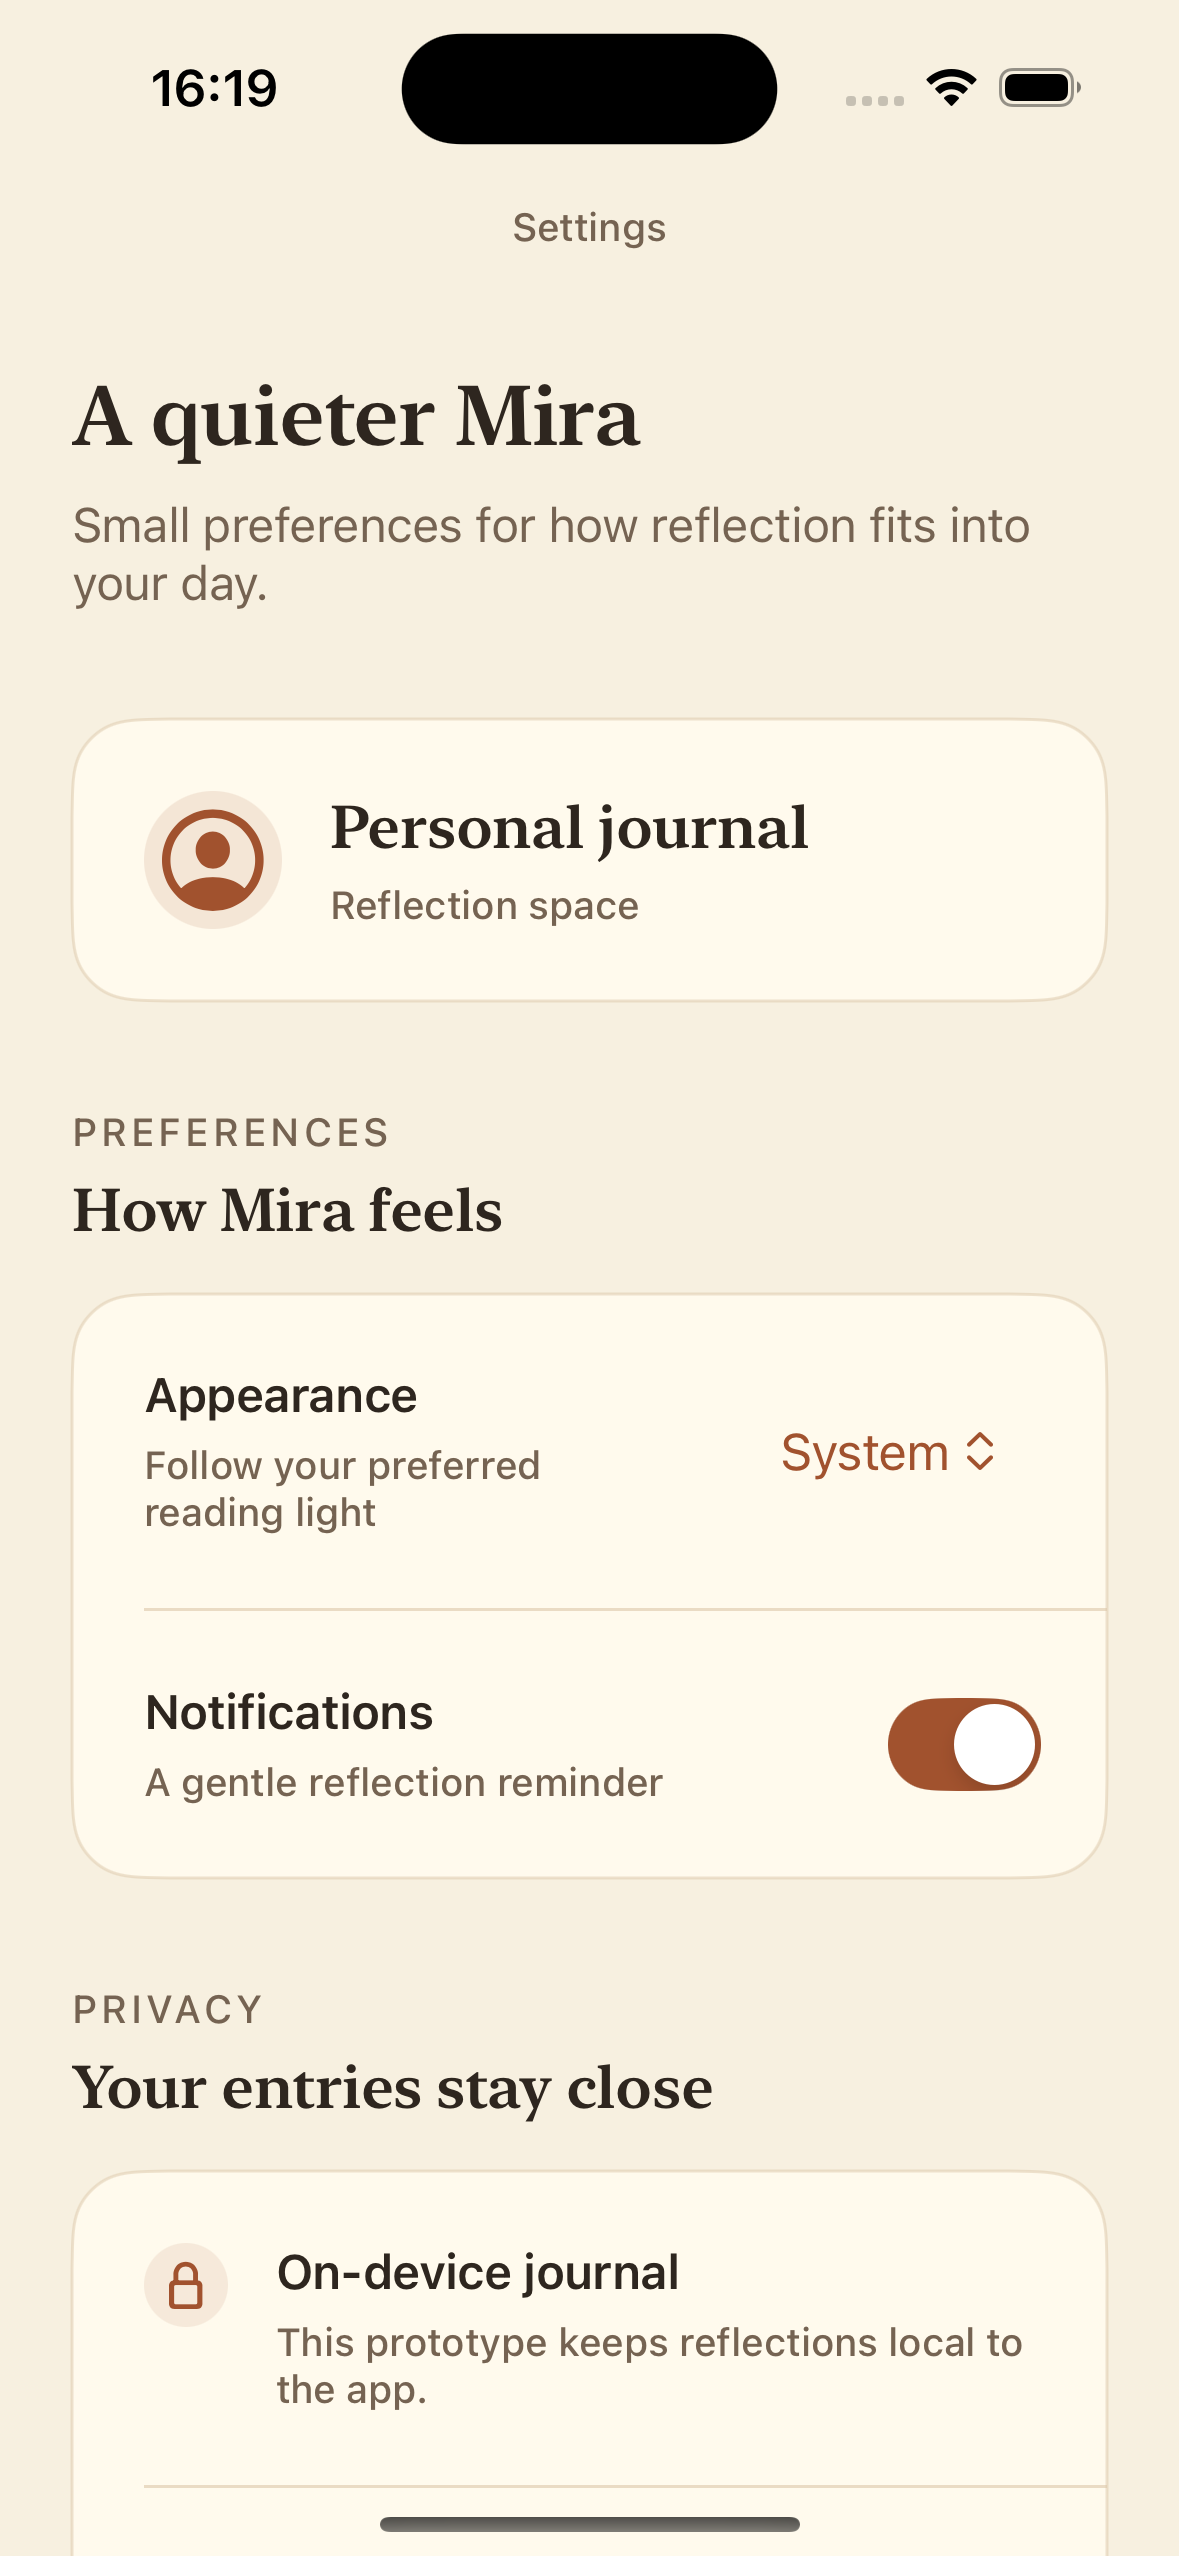
\includegraphics[width=0.28\textwidth]{assets/task001-codex-settings.png}
  \caption{Task 001 Codex Settings screenshot. The run passed automation but failed product-quality review.}
\end{figure}

\section{Case Study 2: Small Diff, Meaningful Taste Difference}

Task 002 asked agents to improve the Journal empty state. Both Codex and Hermes changed one file, passed build/tests, and shipped plausible empty states. The difference was subtle but meaningful.

\begin{center}
\begin{tabular}{lccccc}
\toprule
\textbf{Agent} & \textbf{Files} & \textbf{+/-} & \textbf{Token refs} & \textbf{Score} & \textbf{Ship} \\
\midrule
Codex & 1 & 46/7 & 20 & 21.7/24 & yes-with-polish \\
Hermes & 1 & 35/5 & 17 & 22.8/24 & yes \\
\bottomrule
\end{tabular}
\end{center}

Hermes reviewed slightly better because the copy and hierarchy felt calmer and less constructed. This is exactly the kind of product nuance that conventional automation struggles to detect.

\begin{figure}[H]
  \centering
  \begin{subfigure}{0.42\textwidth}
    \centering
    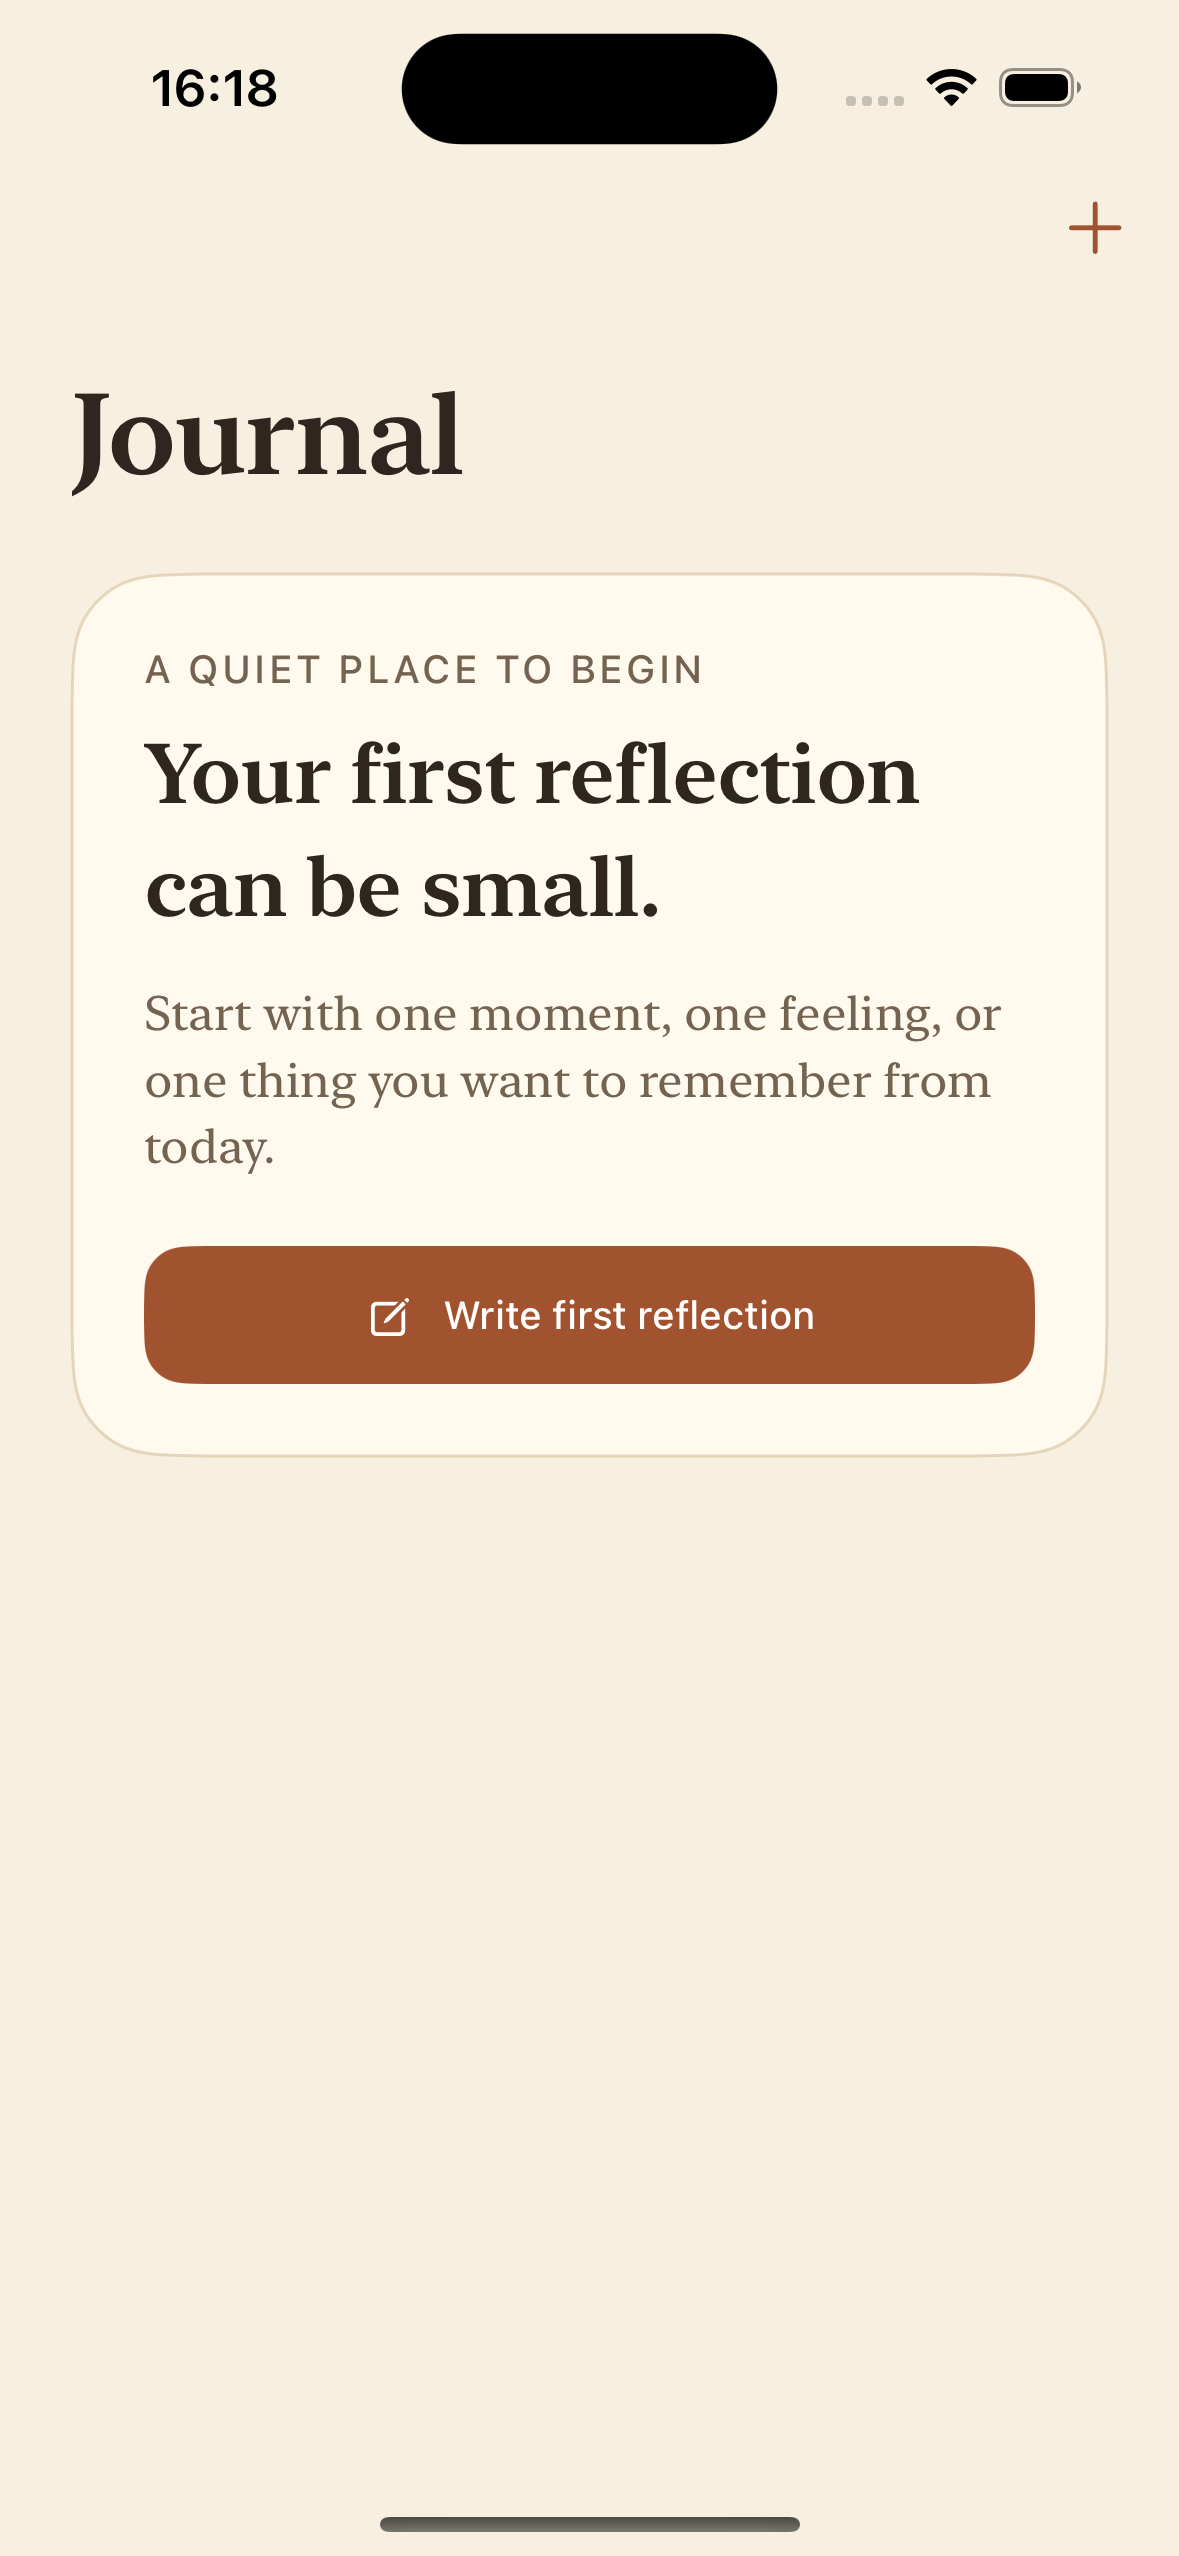
\includegraphics[width=0.9\linewidth]{assets/task002-codex-empty.png}
    \caption{Codex, 21.7/24}
  \end{subfigure}
  \hfill
  \begin{subfigure}{0.42\textwidth}
    \centering
    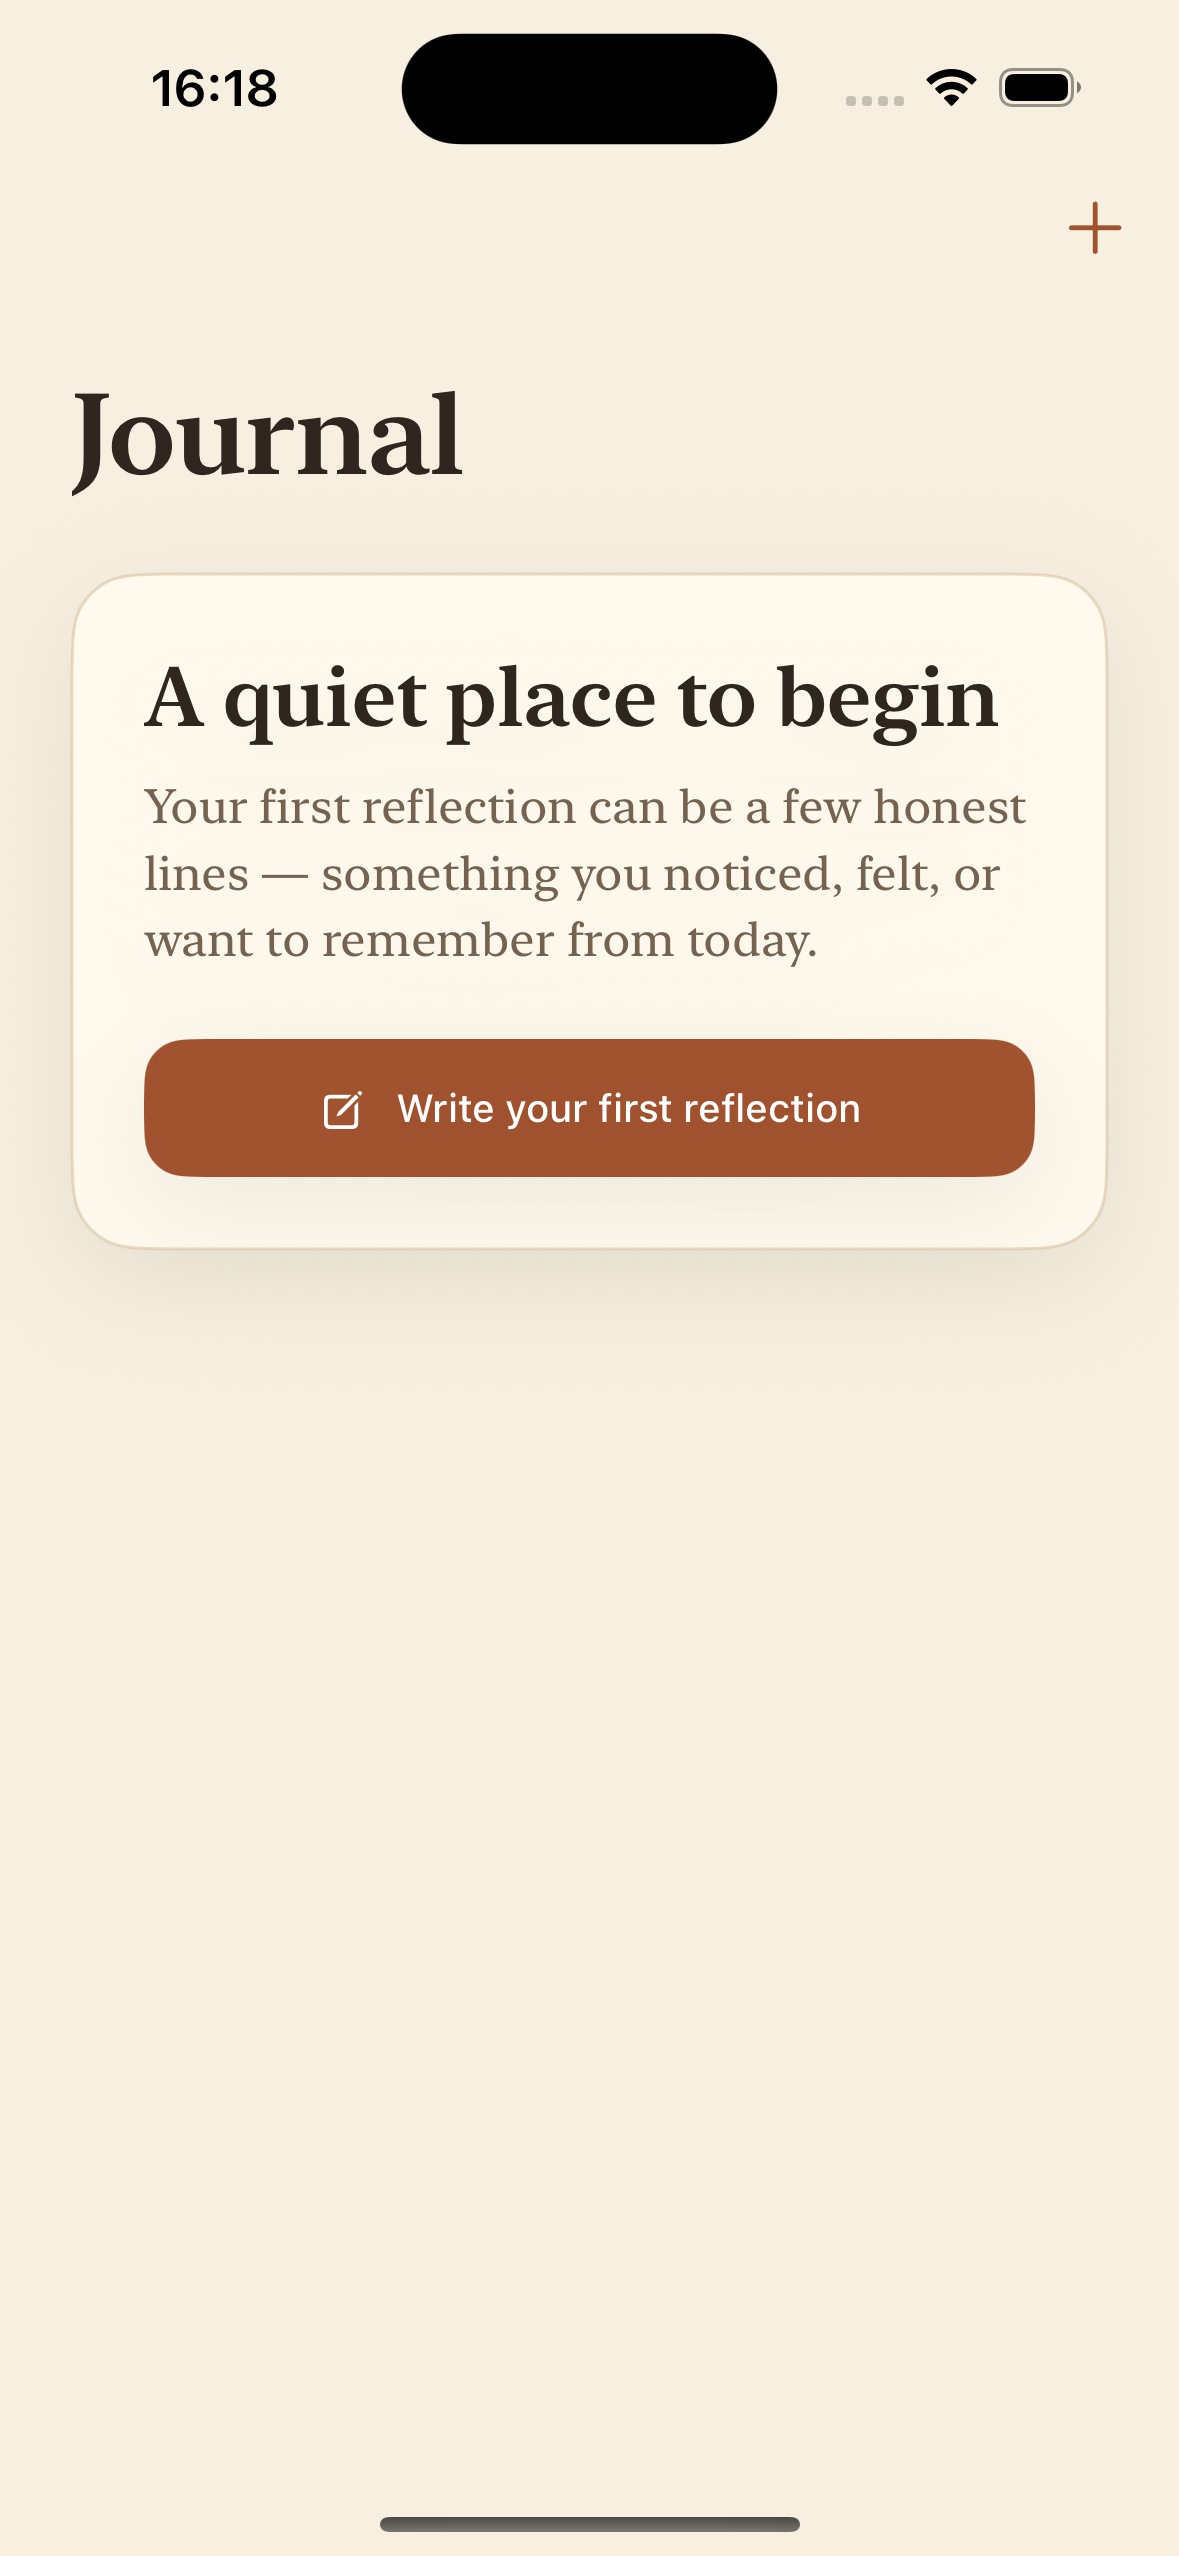
\includegraphics[width=0.9\linewidth]{assets/task002-hermes-empty.png}
    \caption{Hermes, 22.8/24}
  \end{subfigure}
  \caption{Task 002 empty-state comparison. Both runs passed automation; human review separated copy and hierarchy nuance.}
\end{figure}

\section{Case Study 3: Design-System Hygiene}

Task 003 asked agents to improve Mira's dark-mode fidelity. Both Codex and Hermes were valid comparable product runs. Both passed build/tests, stayed within allowed paths, and produced reasonable dark-mode improvements. The difference was design-system discipline.

\begin{center}
\begin{tabular}{lcccccc}
\toprule
\textbf{Agent} & \textbf{Files} & \textbf{+/-} & \textbf{Raw colors} & \textbf{Token refs} & \textbf{Score} & \textbf{Ship} \\
\midrule
Codex & 4 & 64/22 & 0 & 37 & 23.0/24 & yes \\
Hermes & 5 & 45/17 & 28 & 39 & 20.5/24 & yes-with-cleanup \\
\bottomrule
\end{tabular}
\end{center}

Codex centralized mood color selection through the design system and removed raw component colors. Hermes had one idea worth borrowing --- stronger shared dark-mode surface borders --- but left raw dynamic \texttt{UIColor} values in mood styling. The evaluator flagged 28 raw color usages, and human review treated that as a real maintainability smell.

\begin{figure}[H]
  \centering
  \begin{subfigure}{0.42\textwidth}
    \centering
    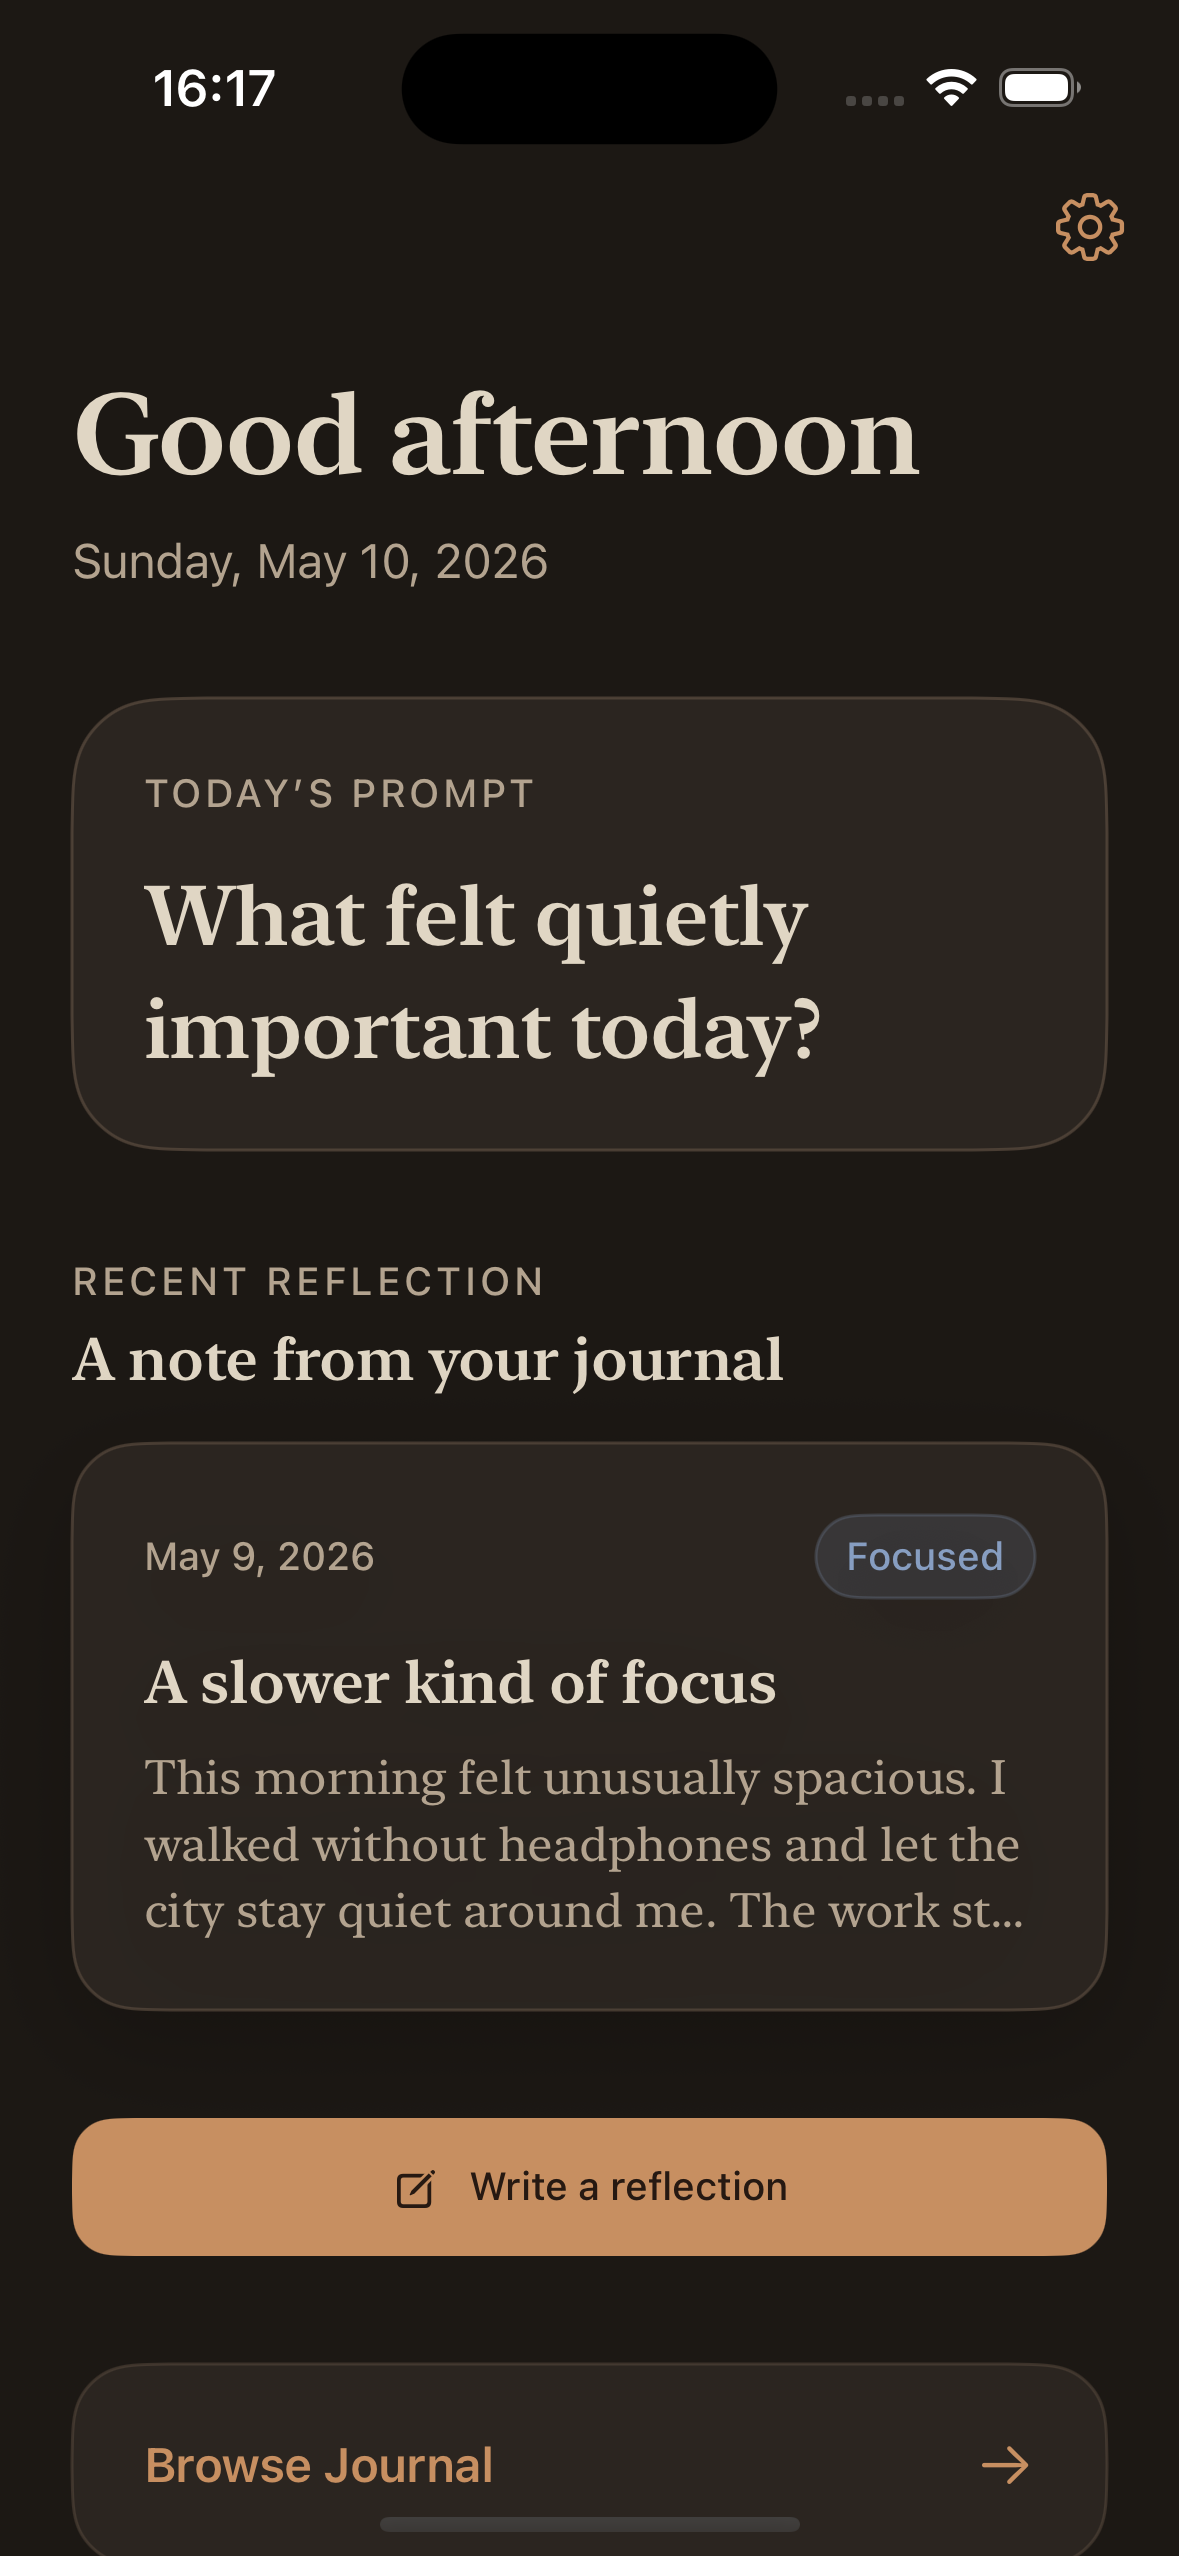
\includegraphics[width=0.9\linewidth]{assets/task003-codex-dark-today.png}
    \caption{Codex dark mode, 23/24}
  \end{subfigure}
  \hfill
  \begin{subfigure}{0.42\textwidth}
    \centering
    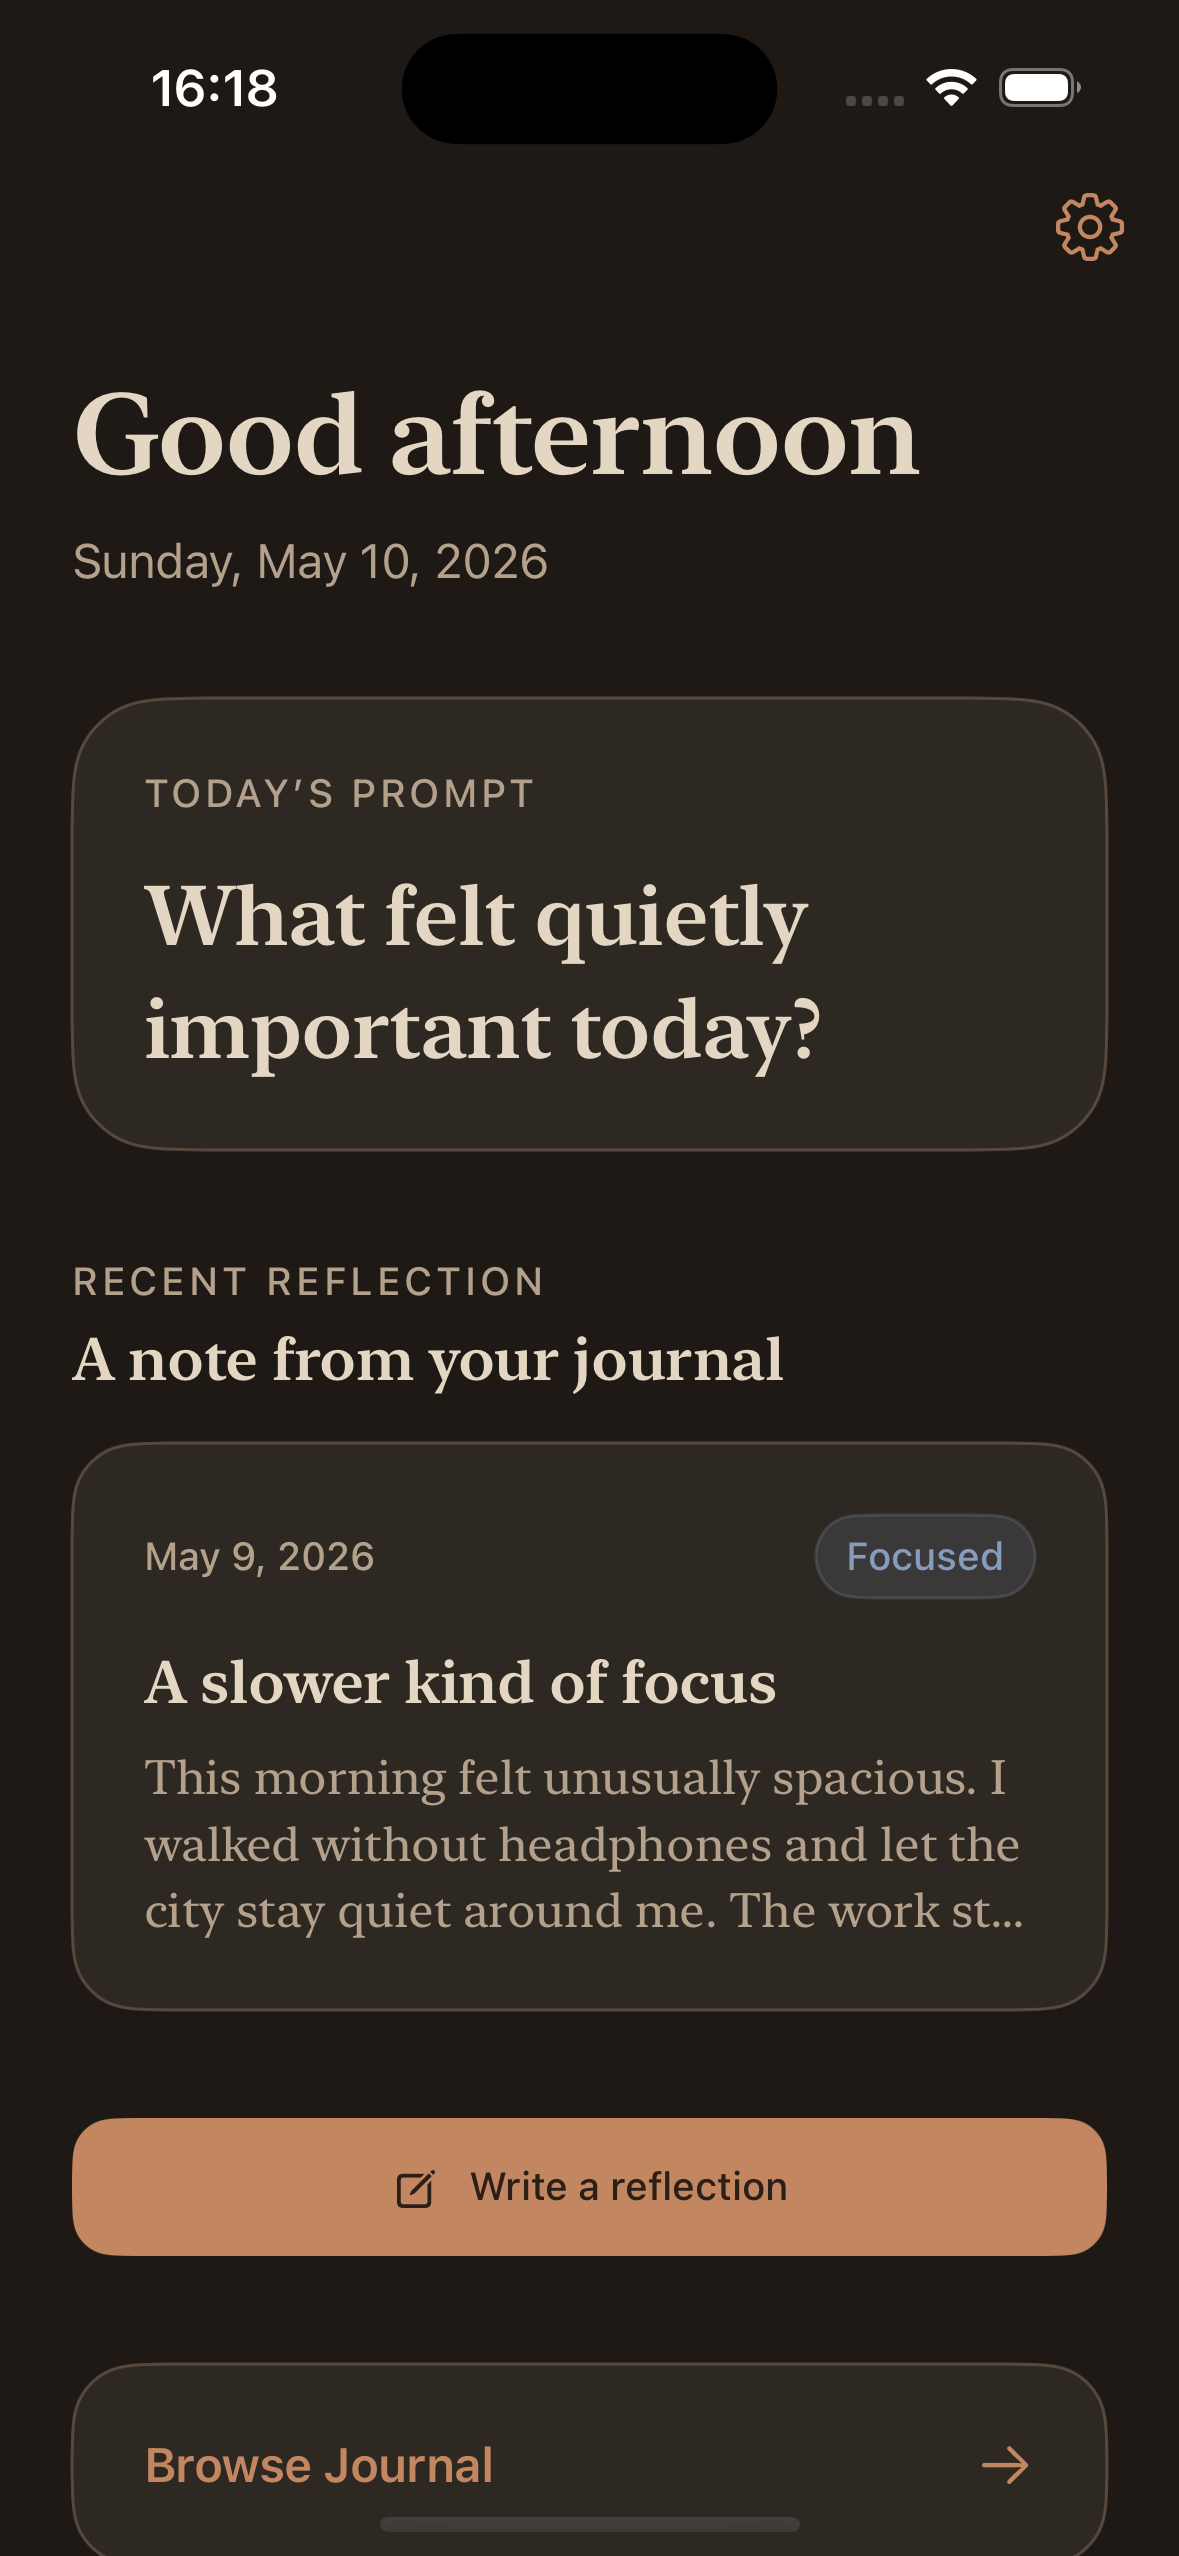
\includegraphics[width=0.9\linewidth]{assets/task003-hermes-dark-today.png}
    \caption{Hermes dark mode, 20.5/24}
  \end{subfigure}
  \caption{Task 003 dark-mode comparison. Both agents improved the app; the winning run preserved design-token ownership more cleanly.}
\end{figure}

\section{Discussion}

TasteBench v0 suggests that coding-agent evaluation needs multiple lanes:

\begin{itemize}
  \item \textbf{Correctness:} Does it build, test, and satisfy the task?
  \item \textbf{Reviewability:} Is the diff narrow, inspectable, and easy to reason about?
  \item \textbf{Product taste:} Does it preserve the app's voice, hierarchy, restraint, and native feel?
  \item \textbf{System discipline:} Does it respect shared tokens and design primitives instead of scattering one-off implementation decisions?
\end{itemize}

The most important lesson is that product taste can be made explicit enough to review. It is not fully automatable, but it can be made visible through rubrics, screenshots, diffs, and structured human review.

\section{Limitations}

TasteBench v0 is intentionally small. It currently includes one app domain, a small number of tasks, and a single human-review perspective. Scores should be treated as early signal, not universal claims about agent quality. Future iterations should add repeated runs, more reviewers, more product surfaces, richer interaction/video capture, and calibration across different task types.

\section{Next Work}

The next benchmark task should test Mira's core writing loop: \textbf{New Entry Writing Flow Polish}. This would evaluate keyboard behavior, save affordance, disabled states, emotional tone, and interaction smoothness. Future dashboard work should add screenshot zoom, richer case-study pages, and a public-facing portfolio report.

\section{Public Framing}

A concise public version of the TasteBench v0 result:

\begin{quote}
I built TasteBench: a benchmark for whether AI coding agents can make product-quality app changes, not just code that builds. In the first snapshot, 6/6 runs passed build and tests, but one still failed human product review. The signal: product taste shows up in copy, hierarchy, restraint, interaction feel, and design-system hygiene.
\end{quote}

\end{document}
